\section{Backend}
\subsection{Technologies and libraries}
\subsubsection{NodeJs}
Node.js is an open-source\textsubscript{\textbf{G}}, cross-platform, backend\textsubscript{\textbf{G}} JavaScript runtime environment that runs on the
V8 engine and executes JavaScript code outside a web browser. Node.js lets developers use JavaScript
to write command line tools and for server-side scripting—running scripts server-side to produce
dynamic web page content before the page is sent to the user’s web browser. Consequently, Node.js
represents a "JavaScript everywhere" paradigm, unifying web-application development around a single
programming language, rather than different languages for server-side and client-side scripts.
\begin{itemize}
    \item \textbf{Used Version: 14.17.0}
    \item \textbf{Link: \url{https://nodejs.org/}}
\end{itemize}
\subsubsection{Serverless Framework}
The Serverless Framework is a free and open-source web framework\textsubscript{\textbf{G}} written using Node.js. Serverless is the first
framework developed for building applications on AWS Lambda, a serverless\textsubscript{\textbf{G}} computing platform provided
by Amazon as a part of Amazon Web Services.
\begin{itemize}
    \item \textbf{Used Version: 2.48.0}
    \item \textbf{Link: \url{https://www.serverless.com/}}
\end{itemize}
\subsubsection{Amazon DynamoDB}
Amazon DynamoDB is a fully managed, multi-region, multi-active, durable, proprietary NoSQL\textsubscript{\textbf{G}} database service that supports key-value
and document data structures and is offered by Amazon.com as part of the Amazon Web Services
portfolio.
\begin{itemize}
    \item \textbf{Link: \url{https://aws.amazon.com/dynamodb/}}
\end{itemize}
\subsubsubsection{Chai}
Chai is a BDD / TDD assertion library for node\textsubscript{\textbf{G}} and the browser that can be delightfully paired with any javascript testing framework.
\begin{itemize}
    \item \textbf{Used Version: 4.3.4}
    \item \textbf{Link: \url{https://www.chaijs.com/}}
\end{itemize}
\subsection{Architecture}
\subsubsection{External services}
\subsubsubsection{Amazon API Gateway}
Amazon API Gateway is a fully managed service that makes it easy for developers to create, publish, maintain, monitor,
and secure APIs at any scale. APIs act as the "front door" for applications to access data, business logic,
or functionality from your backend\textsubscript{\textbf{G}} services. Using API Gateway, you can create RESTful APIs\textsubscript{\textbf{G}} and WebSocket APIs\textsubscript{\textbf{G}} that
enable real-time two-way communication applications. API Gateway supports containerized and serverless workloads,
as well as web applications.
\begin{itemize}
    \item \textbf{Link: \url{https://aws.amazon.com/api-gateway/}}
\end{itemize}
\subsubsubsection{Amazon Cognito}
Amazon Cognito lets you add user sign-up, sign-in, and access control to your web and mobile apps quickly and easily.
Amazon Cognito scales to millions of users and supports sign-in with social identity providers, such as Apple,
Facebook, Google, and Amazon, and enterprise identity providers via SAML 2.0 and OpenID Connect.
\begin{itemize}
    \item \textbf{Link: \url{https://aws.amazon.com/cognito/}}
\end{itemize}
\subsubsubsection{AWS Lambda}
AWS Lambda is an event-driven, serverless\textsubscript{\textbf{G}} computing platform provided by Amazon as a part of Amazon Web Services.
It is a computing service that runs code in response to events and automatically manages the computing resources required by that code.
\begin{itemize}
    \item \textbf{Link: \url{https://aws.amazon.com/lambda/}}
\end{itemize}
\subsubsubsection{Amazon S3}
Amazon Simple Storage Service (Amazon S3) is an object storage service that offers industry-leading scalability,
data availability, security, and performance.
\begin{itemize}
    \item \textbf{Link: \url{https://aws.amazon.com/s3/}}
\end{itemize}
\subsubsubsection{Amazon SNS}
Amazon Simple Notification Service (Amazon SNS) is a fully managed messaging service for both application-to-application (A2A) and application-to-person (A2P) communication.
\begin{itemize}
    \item \textbf{Link: \url{https://aws.amazon.com/sns/}}
\end{itemize}
\subsubsubsection{Amazon SQS}
Amazon Simple Queue Service (SQS) is a fully managed message queuing service that enables you to decouple and scale microservices, distributed systems, and serverless applications.
\begin{itemize}
    \item \textbf{Link: \url{https://aws.amazon.com/sqs/}}
\end{itemize}
\subsubsubsection{Amazon SES}
Amazon Simple Email Service (SES) is a cost-effective, flexible, and scalable email service that enables developers to send mail from within any application.
\begin{itemize}
    \item \textbf{Link: \url{https://aws.amazon.com/ses/}}
\end{itemize}
\subsubsubsection{Amazon Cloudwatch}
Amazon CloudWatch is a monitoring and observability service built for DevOps\textsubscript{\textbf{G}} engineers, developers, site reliability engineers (SREs), and IT managers.
\begin{itemize}
    \item \textbf{Link: \url{https://aws.amazon.com/cloudwatch/}}
\end{itemize}

\subsection{General description}
The platform uses a microservices\textsubscript{\textbf{G}} architecture; each service contains the code necessary for each lambda function, within the relative directory.
The functionalities provided by the platform permitted to identify the following domains:
\begin{itemize}
    \item \textbf{Carts};
    \item \textbf{Products};
    \item \textbf{Orders};
    \item \textbf{Tags};
    \item \textbf{Categories}.
\end{itemize}
The architecture is based on the following microservices\textsubscript{\textbf{G}}:
\begin{itemize}
    \item \textbf{Carts service};
    \item \textbf{Products service};
    \item \textbf{Orders service};
    \item \textbf{Tags service};
    \item \textbf{Categories service}.
\end{itemize}
Microservices\textsubscript{\textbf{G}} are independently deployable and allow for more team autonomy, permitting to manage development in decentralized way.
\pagebreak
\subsection{Microservices structure}
\subsubsection{Carts service}
\begin{figure}[!h]
    \vspace{5px}
    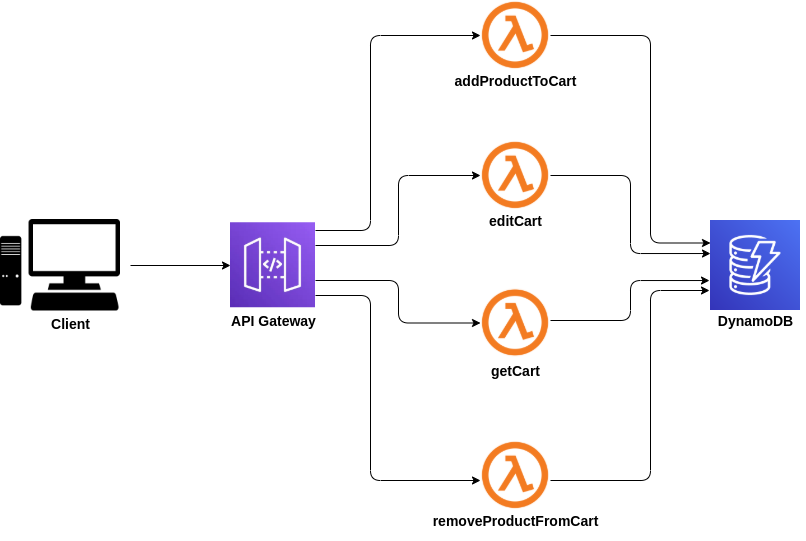
\includegraphics[scale=0.5]{../../../../Images/Diagrammi/maintainerManual/cartService.png}
    \centering
    \caption{Carts service}
\end{figure}
\pagebreak
This microservice\textsubscript{\textbf{G}} allows the user to:
\begin{itemize}
    \item Add a product to the cart;
    \item Remove a product from the cart;
    \item Modify the quantity of the items in the cart;
    \item View the items in the cart;
    \item Delete the cart;
    \item Check-out.
\end{itemize}
The Carts service allows the user to manage their shopping cart.
To check the consistency of the data, functions are called from the SQS service to maintain consistency when a product is changed or deleted.
In addition, these functions, through the use of the SES service, allow customers to be notified via email of the change in their cart.
Stripe is used as an external service to manage checkout, which allows you to access the session for payment of the order. Once the checkout is complete, the createCheckout lambda sends a message through the SNS service with the order data in order to create the same through the appropriate service.
\pagebreak
\subsubsection{Products service}
\begin{figure}[!h]
    \vspace{5px}
    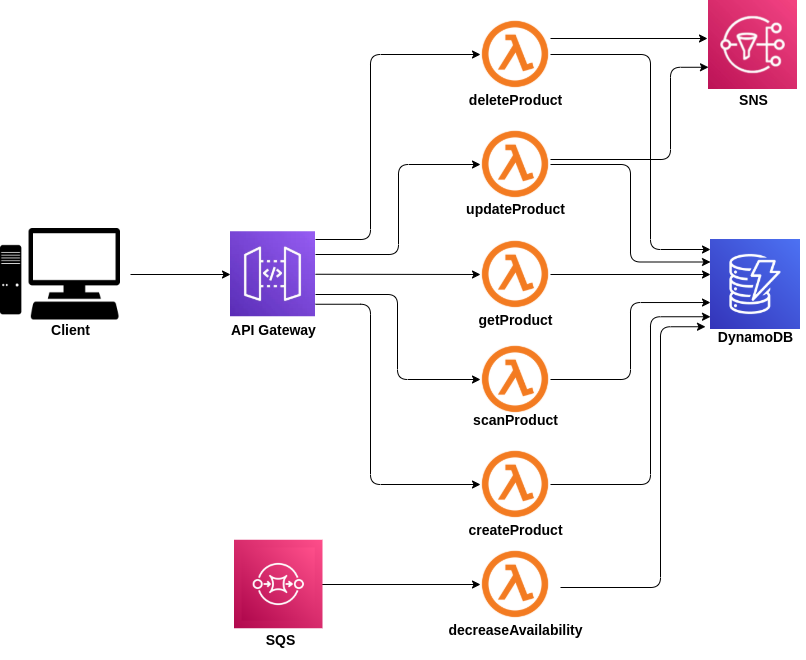
\includegraphics[scale=0.5]{../../../../Images/Diagrammi/maintainerManual/productService.png}
    \centering
    \caption{Products service}
\end{figure}
This microservice\textsubscript{\textbf{G}} allows the vendor to:
\begin{itemize}
    \item Create a new product;
    \item Delete a product;
    \item Modify some information about a product.
\end{itemize}
This microservice\textsubscript{\textbf{G}} also allows any user to:
\begin{itemize}
    \item View the product details;
    \item Find a specific product using filters;
\end{itemize}
The Products service allows the vendor to manage the products of their store. It also allows any user to view them both in the list with the possibility of filtering them and in detail. When a product is deleted or modified, messages are sent via the SNS service, to update all the carts and report any changes to the product present in them. Furthermore, through an SQS queue, when an order is placed the quantity available for the purchased products is decreased.
\pagebreak
\subsubsection{Orders service}
\begin{figure}[!h]
    \vspace{5px}
    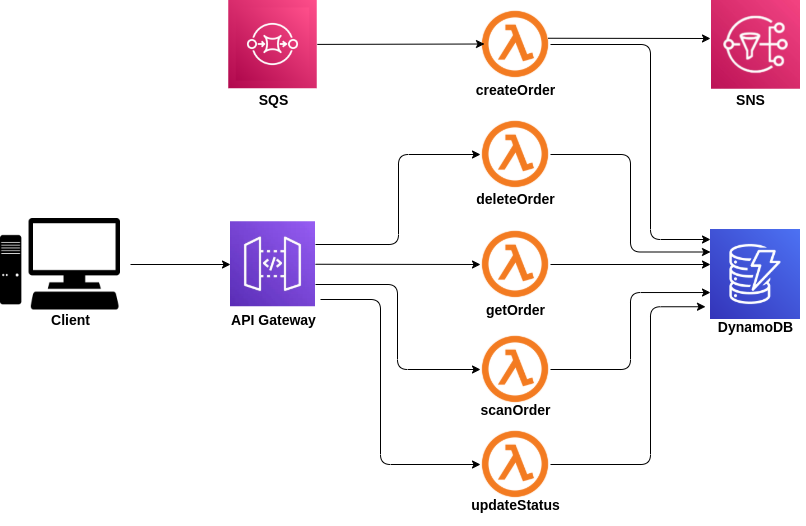
\includegraphics[scale=0.5]{../../../../Images/Diagrammi/maintainerManual/orderService.png}
    \centering
    \caption{Orders service}
\end{figure}
This microservice\textsubscript{\textbf{G}} allows the user to:
\begin{itemize}
    \item Create a new order;
    \item Delete a order;
    \item View the order details;
    \item Find a specific order using filters.
\end{itemize}
The Orders service allows the user to manage and place their orders.
The order with the data received after checkout is created through an SQS queue. After the order has been paid for, messages are sent via the SNS service to decrease the quantity of products available.
\pagebreak
\subsubsection{Tags service}
\begin{figure}[!h]
    \vspace{5px}
    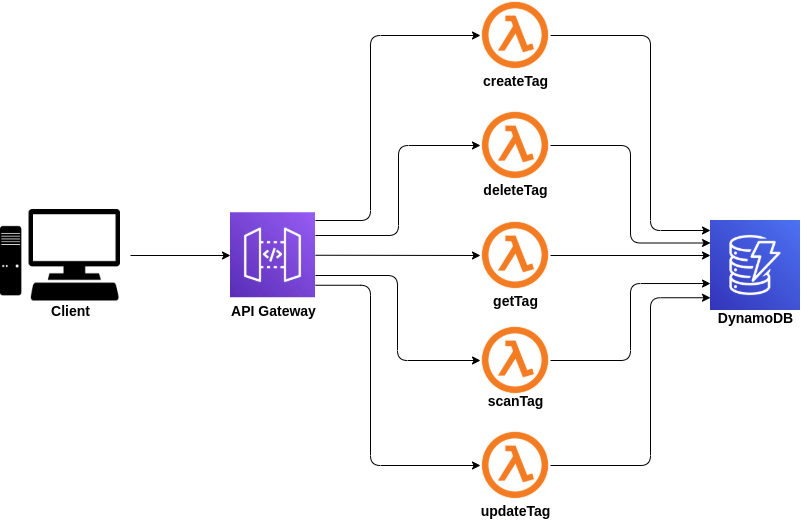
\includegraphics[scale=0.5]{../../../../Images/Diagrammi/maintainerManual/tagsService.png}
    \centering
    \caption{Tags service}
\end{figure}
This microservice\textsubscript{\textbf{G}} allows the vendor to:
\begin{itemize}
    \item Create a new tag;
    \item Delete a tag;
    \item Modify information about a tag.
\end{itemize}
This microservice\textsubscript{\textbf{G}} also allows any user to:
\begin{itemize}
    \item View the tag;
    \item Find a specific tag using filters.
\end{itemize}
The Products service allows the vendor to manage the tags of their store. It also allows any user to view and filter them.
\pagebreak
\subsubsection{Categories service}
\begin{figure}[!h]
    \vspace{5px}
    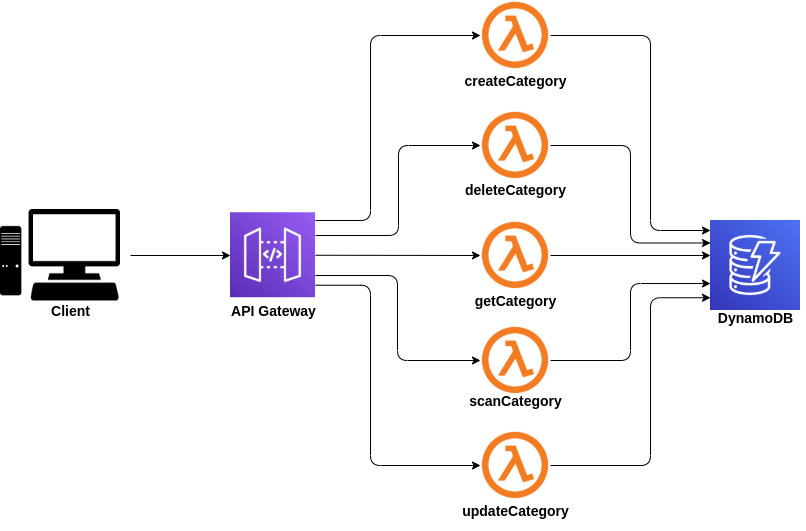
\includegraphics[scale=0.5]{../../../../Images/Diagrammi/maintainerManual/categoriesService.png}
    \centering
    \caption{Categories service}
\end{figure}
This microservice\textsubscript{\textbf{G}} allows the vendor to:
\begin{itemize}
    \item Create a new category;
    \item Delete a category;
    \item Modify information about a category.
\end{itemize}
This microservice\textsubscript{\textbf{G}} also allows any user to:
\begin{itemize}
    \item View the category;
    \item Find a specific category using filters.
\end{itemize}
The Products service allows the vendor to manage the categories of their store. It also allows any user to view and filter them.

\pagebreak
\subsection{Sequence diagrams}
The following sequence diagrams describe the main operations that can be carried out inside the platform:
\subsubsection{Create product}
\begin{figure}[!h]
    \vspace{5px}
    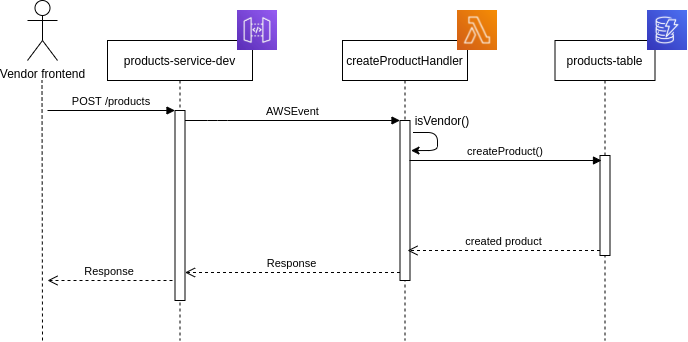
\includegraphics[scale=0.5]{../../../../Images/Diagrammi/maintainerManual/createProductSequence.png}
    \centering
    \caption{sequence diagram for creating a product}
\end{figure}
The diagram represents the sequence of operations necessary to create a product, the \textit{isVendor()} method is responsible for checking that the user who accesses the creation of the product is a vendor and therefore has access to this functionality.
\pagebreak
\subsubsection{Remove product from cart}
\begin{figure}[!h]
    \vspace{5px}
    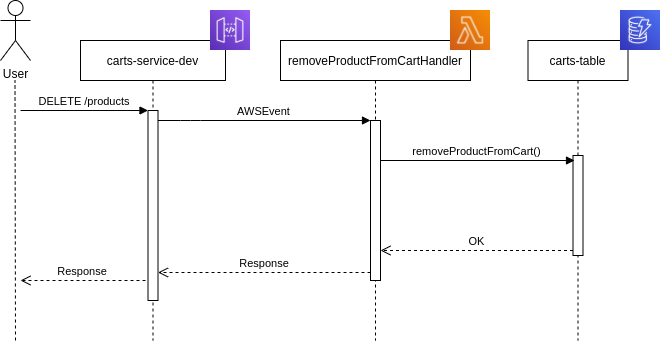
\includegraphics[scale=0.5]{../../../../Images/Diagrammi/maintainerManual/removeProductFromCart.png}
    \centering
    \caption{sequence diagram for removing a product from the cart}
\end{figure}
The diagram represents the sequence of operations required for any user to remove a product from the cart.
\pagebreak
\subsubsection{Create checkout}
\begin{figure}[!h]
    \vspace{5px}
    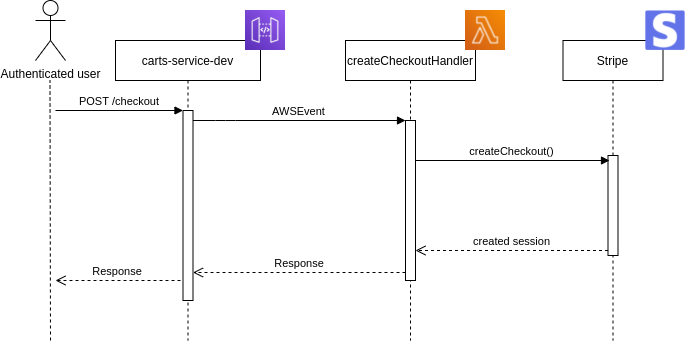
\includegraphics[scale=0.5]{../../../../Images/Diagrammi/maintainerManual/createCheckoutSequence.png}
    \centering
    \caption{sequence diagram for checking out}
\end{figure}
The diagram represents the sequence of operations necessary for the checkout with consequent payment of the order. This feature is only available if the user is authenticated and uses Stripe as an external service to proceed with the payment of the order.
\pagebreak
\subsubsection{Scan tag}
\begin{figure}[!h]
    \vspace{5px}
    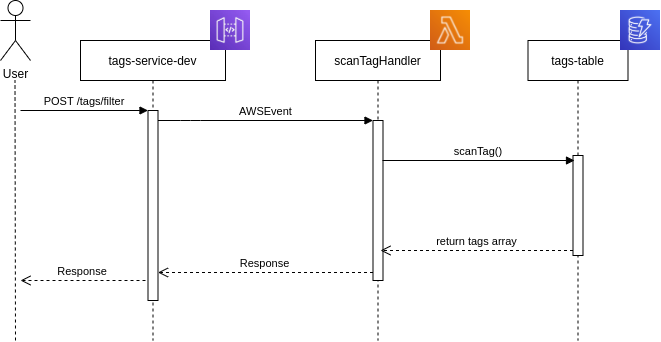
\includegraphics[scale=0.5]{../../../../Images/Diagrammi/maintainerManual/scanTagSequence.png}
    \centering
    \caption{sequence diagram for scanning a tag}
\end{figure}
The diagram represents the sequence of operations required to scan the tags, using filters. this feature can be used by any user.
\pagebreak
\subsubsection{Update category}
\begin{figure}[!h]
    \vspace{5px}
    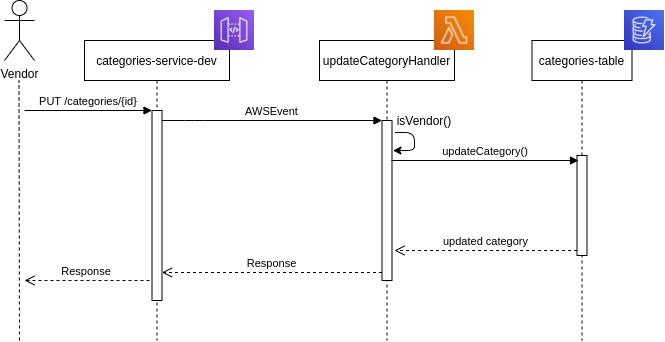
\includegraphics[scale=0.5]{../../../../Images/Diagrammi/maintainerManual/updateCategorySequence.png}
    \centering
    \caption{sequence diagram for updating a category}
\end{figure}
The diagram represents the sequence of operations required to update a category. This function is only accessible by a vendor, for this reason there is the \textit{isVendor()} method to check that the user who accesses it is actually a vendor.
\pagebreak
\subsubsection{Get product}
\begin{figure}[!h]
    \vspace{5px}
    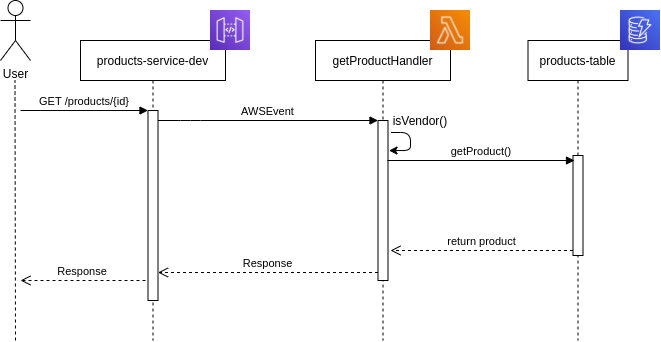
\includegraphics[scale=0.5]{../../../../Images/Diagrammi/maintainerManual/getProductSequence.png}
    \centering
    \caption{sequence diagram for getting a product}
\end{figure}
The diagram represents the sequence of operations necessary to obtain information regarding a product, this function is accessible to any user. The \textit{isVendor()} function checks the type of user and returns different product information depending on the case.
